\section{eo\-Uniform\-Mutation$<$ EOT $>$ Class Template Reference}
\label{classeo_uniform_mutation}\index{eoUniformMutation@{eoUniformMutation}}
eo\-Uniform\-Mutation --$>$ changes all values of the std::vector by uniform choice with range epsilon with probability p\_\-change per variable  


{\tt \#include $<$Tutorial/eo\-Real\-Op.h$>$}

Inheritance diagram for eo\-Uniform\-Mutation$<$ EOT $>$::\begin{figure}[H]
\begin{center}
\leavevmode
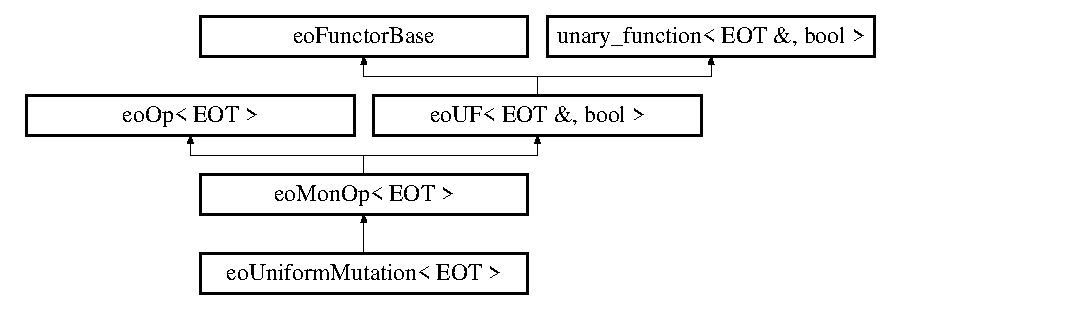
\includegraphics[height=3.71476cm]{classeo_uniform_mutation}
\end{center}
\end{figure}
\subsection*{Public Member Functions}
\begin{CompactItemize}
\item 
{\bf eo\-Uniform\-Mutation} (const double \&\_\-epsilon, const double \&\_\-p\_\-change=1.0)
\begin{CompactList}\small\item\em Constructor without bounds == unbounded variables :-) not very clean, but who's doing unbounded optimization anyway? and it's there mostly for backward compatibility. \item\end{CompactList}\item 
{\bf eo\-Uniform\-Mutation} ({\bf eo\-Real\-Vector\-Bounds} \&\_\-bounds, const double \&\_\-epsilon, const double \&\_\-p\_\-change=1.0)
\begin{CompactList}\small\item\em Constructor with bounds. \item\end{CompactList}\item 
{\bf eo\-Uniform\-Mutation} ({\bf eo\-Real\-Vector\-Bounds} \&\_\-bounds, const std::vector$<$ double $>$ \&\_\-epsilon, const std::vector$<$ double $>$ \&\_\-p\_\-change)
\begin{CompactList}\small\item\em Constructor with bounds. \item\end{CompactList}\item 
virtual std::string {\bf class\-Name} () const \label{classeo_uniform_mutation_a3}

\begin{CompactList}\small\item\em The class name. \item\end{CompactList}\item 
bool {\bf operator()} ({\bf EOT} \&\_\-eo)
\begin{CompactList}\small\item\em Do it! \item\end{CompactList}\end{CompactItemize}
\subsection*{Private Attributes}
\begin{CompactItemize}
\item 
bool {\bf homogeneous}\label{classeo_uniform_mutation_r0}

\item 
{\bf eo\-Real\-Vector\-Bounds} \& {\bf bounds}\label{classeo_uniform_mutation_r1}

\item 
std::vector$<$ double $>$ {\bf epsilon}\label{classeo_uniform_mutation_r2}

\item 
std::vector$<$ double $>$ {\bf p\_\-change}\label{classeo_uniform_mutation_r3}

\end{CompactItemize}


\subsection{Detailed Description}
\subsubsection*{template$<$class EOT$>$ class eo\-Uniform\-Mutation$<$ EOT $>$}

eo\-Uniform\-Mutation --$>$ changes all values of the std::vector by uniform choice with range epsilon with probability p\_\-change per variable 



Definition at line 45 of file eo\-Real\-Op.h.

\subsection{Constructor \& Destructor Documentation}
\index{eoUniformMutation@{eo\-Uniform\-Mutation}!eoUniformMutation@{eoUniformMutation}}
\index{eoUniformMutation@{eoUniformMutation}!eoUniformMutation@{eo\-Uniform\-Mutation}}
\subsubsection{\setlength{\rightskip}{0pt plus 5cm}template$<$class EOT$>$ {\bf eo\-Uniform\-Mutation}$<$ {\bf EOT} $>$::{\bf eo\-Uniform\-Mutation} (const double \& {\em \_\-epsilon}, const double \& {\em \_\-p\_\-change} = {\tt 1.0})\hspace{0.3cm}{\tt  [inline]}}\label{classeo_uniform_mutation_a0}


Constructor without bounds == unbounded variables :-) not very clean, but who's doing unbounded optimization anyway? and it's there mostly for backward compatibility. 

\begin{Desc}
\item[Parameters:]
\begin{description}
\item[{\em \_\-epsilon}]the range for uniform nutation \item[{\em \_\-p\_\-change}]the probability to change a given coordinate \end{description}
\end{Desc}


Definition at line 56 of file eo\-Real\-Op.h.\index{eoUniformMutation@{eo\-Uniform\-Mutation}!eoUniformMutation@{eoUniformMutation}}
\index{eoUniformMutation@{eoUniformMutation}!eoUniformMutation@{eo\-Uniform\-Mutation}}
\subsubsection{\setlength{\rightskip}{0pt plus 5cm}template$<$class EOT$>$ {\bf eo\-Uniform\-Mutation}$<$ {\bf EOT} $>$::{\bf eo\-Uniform\-Mutation} ({\bf eo\-Real\-Vector\-Bounds} \& {\em \_\-bounds}, const double \& {\em \_\-epsilon}, const double \& {\em \_\-p\_\-change} = {\tt 1.0})\hspace{0.3cm}{\tt  [inline]}}\label{classeo_uniform_mutation_a1}


Constructor with bounds. 

\begin{Desc}
\item[Parameters:]
\begin{description}
\item[{\em \_\-bounds}]an {\bf eo\-Real\-Vector\-Bounds}{\rm (p.\,\pageref{classeo_real_vector_bounds})} that contains the bounds \item[{\em \_\-epsilon}]the range for uniform mutation - a double to be scaled \item[{\em \_\-p\_\-change}]the one probability to change all coordinates \end{description}
\end{Desc}


Definition at line 66 of file eo\-Real\-Op.h.

References eo\-Real\-Base\-Vector\-Bounds::is\-Bounded(), and eo\-Real\-Base\-Vector\-Bounds::range().\index{eoUniformMutation@{eo\-Uniform\-Mutation}!eoUniformMutation@{eoUniformMutation}}
\index{eoUniformMutation@{eoUniformMutation}!eoUniformMutation@{eo\-Uniform\-Mutation}}
\subsubsection{\setlength{\rightskip}{0pt plus 5cm}template$<$class EOT$>$ {\bf eo\-Uniform\-Mutation}$<$ {\bf EOT} $>$::{\bf eo\-Uniform\-Mutation} ({\bf eo\-Real\-Vector\-Bounds} \& {\em \_\-bounds}, const std::vector$<$ double $>$ \& {\em \_\-epsilon}, const std::vector$<$ double $>$ \& {\em \_\-p\_\-change})\hspace{0.3cm}{\tt  [inline]}}\label{classeo_uniform_mutation_a2}


Constructor with bounds. 

\begin{Desc}
\item[Parameters:]
\begin{description}
\item[{\em \_\-bounds}]an {\bf eo\-Real\-Vector\-Bounds}{\rm (p.\,\pageref{classeo_real_vector_bounds})} that contains the bounds \item[{\em \_\-epsilon}]the VECTOR of ranges for uniform mutation \item[{\em \_\-p\_\-change}]the VECTOR of probabilities for each coordinates \end{description}
\end{Desc}


Definition at line 83 of file eo\-Real\-Op.h.

\subsection{Member Function Documentation}
\index{eoUniformMutation@{eo\-Uniform\-Mutation}!operator()@{operator()}}
\index{operator()@{operator()}!eoUniformMutation@{eo\-Uniform\-Mutation}}
\subsubsection{\setlength{\rightskip}{0pt plus 5cm}template$<$class EOT$>$ bool {\bf eo\-Uniform\-Mutation}$<$ {\bf EOT} $>$::operator() ({\bf EOT} \& {\em \_\-eo})\hspace{0.3cm}{\tt  [inline, virtual]}}\label{classeo_uniform_mutation_a4}


Do it! 

\begin{Desc}
\item[Parameters:]
\begin{description}
\item[{\em \_\-eo}]The indi undergoing the mutation \end{description}
\end{Desc}


Implements {\bf eo\-UF$<$ EOT \&, bool $>$} {\rm (p.\,\pageref{classeo_u_f_a1})}.

Definition at line 96 of file eo\-Real\-Op.h.

References eo\-Rng::flip(), eo\-Real\-Base\-Vector\-Bounds::is\-Max\-Bounded(), eo\-Real\-Base\-Vector\-Bounds::is\-Min\-Bounded(), eo\-Real\-Base\-Vector\-Bounds::maximum(), eo\-Real\-Base\-Vector\-Bounds::minimum(), and eo\-Rng::uniform().

The documentation for this class was generated from the following file:\begin{CompactItemize}
\item 
eo\-Real\-Op.h\end{CompactItemize}
